\chapter{Sjenčanje}
U fazi sjenčanja, ujedno i posljednjoj fazi ovoga rada, cilj je bio dodati atribute kuglicama kako bi rad izgledao impresivnije. Prije samog korištenja alata za sjenčanje (tzv. Shader) bilo je potrebno promijeniti okolinu u kojoj se rad izvršavao. Do sada, koristili smo OpenGL 1.x, koji je eksperimentalan i ne koristi Shadere za iscrtavanje poligona. S OpenGL-a 1.x, smo iz tog razloga prešli na noviju verziju, OpenGL 3.3 koji nam omogućava korištenje Shadera i nekih naprednijih opcija koje nismo do sada imali.

Iako je noviji, OpenGL 3.3 koristi neke nove principe i modele s kojima se do sada nismo susreli. Zbog toga, morali smo odustati od \emph{GLUT-a}, koji nam je služio za komunikaciju sa operacijskim sustavom (prikaz prozora, korištenje miša i tipkovnice, terminiranje prozora,...). Prešli smo na noviji \emph{GLFW} koji se koristi kod modernijih verzija OpenGL-a. U principu \emph{GLFW} i \emph{GLUT} služe za iste stvari, no \emph{GLFW} je moderniji i pruža nam bolju optimizaciju programa nego stariji \emph{GLUT}. Usprkos tome, \emph{GLFW} nema biblioteke za crtanje sfera, pravokutnika i sl. pa smo morali sami definirati sferu kojom ćemo opisati kuglice. To će biti objašnjeno u narednom poglavlju.
\newpage
\section{Sfera}
Kako smo spomenuli, \emph{GLFW} nema biblioteke kojima možemo nacrtati jednostavne poligone kao što ima \emph{GLUT}. Dakle, do sada korištena funkcija \emph{glutSolidSphere} za crtanje kuglica, više nam nije bilo od koristi i morali smo definirati sami točke kojima ćemo crtati sferu.

Za crtanje sfere postoje generalno 2 načina:
\begin{itemize}
	\item Programsko generiranje točaka, indeksa i normala
	\item Prijenos objekta iz odgovarajućeg formata generiranog u programu za crtanje modela (npr. Blender)
\end{itemize}
U početku je bila velika dilema koji od ova 2 načina odabrati, s obzirom da je svaki od njih imao neke svoje prednosti i mane, no u konačnosti izabrali smo programsko generiranje zbog relativno lakšeg implementiranja od prijenosa objekata. Inače, prijenos objekata iz nekog drugog alata nije sam po sebi težak, no ili zahtjeva dodatne biblioteke (npr. Assimp) ili zahtjeva pisanje programa koji će preuzeti podatke iz formata i postaviti ih u polja koja iscrtavamo.

Kako smo rekli, OpenGL 3.3 za crtanje objekata koristi Shadere. Bez Shadera na sceni nećemo vidjeti ništa, te su oni ti koje objekte prikazuju. Shadere je potrebno posebno kompilirati i to za sada nećemo ovdje prikazivati, nego u kasnijim poglavljima. Za početak koristili smo jednostavne Shadere. Shadere dijelimo na Shadere točaka i Shadere fragmenata\cite{15}. Trenutno nećemo ulaziti u analizu kodova nego ćemo samo prikazati Shadere. Shader točaka definiran je:
\begin{lstlisting}[style = myC++, label = {code:14}, caption = {Jednostavni Shader točaka}]
#version 330 core
layout(location = 0) in vec3 vertexPosition;
// Values that stay constant for the whole mesh.
out vec3 fragmentColor;
void main(){
// Output position of the vertex, in clip space : MVP * position
	gl_Position.xyz =  vertexPosition_modelspace;
	fragmentColor = vertexColor;
}
\end{lstlisting}
Shader fragmenata definiran je kao:
\begin{lstlisting}[style = myC++, label = {code:15}, caption = {Jednostavni Shader fragmenata}]
#version 330 core
// Ouput data
in vec3 fragmentColor;
out vec3 color;

void main()
{
	color = vec3(0.4,0.2,0.7); 
}
\end{lstlisting}

U početku, bilo je vrlo teško krenuti od crtanja same sfere. Trebalo je prvo razumjeti sve strukture koje se koriste u OpenGL-u 3.3 pa smo krenuli prvo od crtanja običnog trokuta korištenjem spomenutih Shadera.

\subsection{Crtanje trokuta}
Crtanje trokuta je prvi korak pri učenju OpenGL-a 3.3 \cite{15}\cite{16}. Na ovom jednostavnom primjeru, mogu se naučiti sve strukture i tipovi podataka koji se koriste prilikom korištenja OpenGL-a 3.3. 

Trokut možemo definirati sa 3 točke. Neka to budu točke:
\begin{itemize}
	\item (-0.5f, -0.5f, 0.0f)
	\item (0.5f, -0.5f, 0.0f)
	\item (0.0f, 0.5f, 0.0f)
\end{itemize}
Vrlo je važno da točke budu definirane točno ovim redom inače ih OpenGL 3.3 neće nacrtati kako smo to htjeli. Ove točke važno je spremiti u strukturu zvanu VBO tj. Vertex Buffer Object. Ova struktura nam omogućava crtanje objekata na grafičkoj kartici, a ne na procesoru\cite{16}. Prije VBO-a definirali smo i Vertex Array Object, no ovdje on nije posebno bitan pa ga nećemo posebno ni spominjati. U nastavku slijedi kod kojime smo generirali VBO i u njega poslali podatke o točkama trokuta\cite{15}.\newpage
\begin{lstlisting}[style = myC++, label = {code:16}, caption = {Generiranje VBO\cite{16}}]
static const float vertices[] = {-0.5f, -0.5f, 0.0f, 0.5f, -0.5f, 0.0f, 0.0f, 0.5f, 0.0f,}; //vertices of triangle
	  
unsigned int VBO;
glGenBuffers(1, &VBO);
glBindBuffer(GL_ARRAY_BUFFER, VBO);
glBufferData(GL_ARRAY_BUFFER, sizeof(vertices), vertices, GL_STATIC_DRAW);
	  
glBindBuffer(GL_ARRAY_BUFFER, VBO);
glVertexAttribPointer(0, 3, GL_FLOAT, GL_FALSE, 3 * sizeof(float), (void *)0);
glEnableVertexAttribArray(0);
glBindBuffer(GL_ARRAY_BUFFER, 0);
\end{lstlisting}
Samo crtanje trokuta izvodi se na:
\begin{lstlisting}[style = myC++, label = {code:16-1}, caption = {Crtanje trokuta\cite{15}}]
do {
	glClear(GL_COLOR_BUFFER_BIT | GL_DEPTH_BUFFER_BIT)
	glUseProgram(Shader);
	glEnableVertexAttribArray(0);
	glBindBuffer(GL_ARRAY_BUFFER, vertexbuffer);
	glDrawArrays(GL_TRIANGLES, 0, 3); // 3 indices starting at 0 -> 1
	glfwSwapBuffers(window);
	glfwPollEvents();
}
\end{lstlisting}

Objašnjenje ovoga koda nećemo raditi, s obzirom da su to funkcije i strukture korištene isključivo sa strane OpenGL-a. Nastavak objašnjenja ovih struktura može se pronaći u \cite{15} i \cite{16}. Na ovakav način dobili smo trokut koji izgleda ovako:\newpage
\begin{figure}[!http]
	\begin{center}
		
\includegraphics[height = 8 cm, width = 8 cm, keepaspectratio = true]{triangle}
		\caption{Trokut u OpenGL-u 3.3}
		\label{fig:29}
		\end{center}
\end{figure}

Idući zadatak bio je ovaj trokut pomicati po prostoru. Ovdje smo umjesto funkcija unutar OpenGL-a koristili \emph{glm} biblioteku matematičkih funkcija koja nam omogućava operacija sa matricama i transformacije u prostoru.

\subsection{Transformacije}

Prije korištenja OpenGL-a 3.3 transformacije smo definirali funkcijama unutar OpenGL-a. S obzirom da smo tada samo crtanje objekata izvršavali na procesoru, ovo je bilo moguće bez problema. Prelaskom na OpenGL 3.3 transformacije smo morali poslati u Shader da bi znali gdje nacrtati objekt.

Svaki objekt ima svoj definirani prostor koji je definiran lokalnim koordinatama\cite{16}. Lokalne koordinate svakog objekta definirane su matricom modela. Transformacijom matrice modela definiramo poziciju svakog objekta unutar cijele scene tj. svijeta. Konačno, matricom pogleda definiramo pogled na svijet tj. koordinate iz kojih imamo pogled na cijelu scenu. U konačnosti definiranjem projekcije definiramo kako ćemo vidjeti stvari na sceni ("Clip space"). Ovo možemo prikazati jednostavnim dijagramom:\newpage
\begin{figure}[!http]
	\begin{center}
		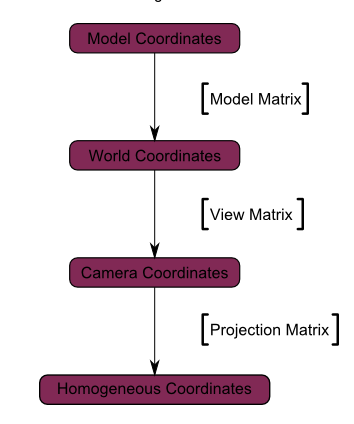
\includegraphics[height = 5 cm, width = 5 cm, keepaspectratio = true]{transformations}
		\caption{Transformacije matrica i koordinata u OpenGL-u\cite{15}}
		\label{fig:30}
	\end{center}
\end{figure}
Umnoškom:
\begin{equation}
	\begin{aligned}
		MVP = Projection Matrix * View Matrix * Model Matrix
	\end{aligned}
\end{equation}
dobili smo transformaciju točaka u prostor koji mi vidimo (ili ne vidimo)\cite{16}. Transformacijom matrice modela (Model Matrix), možemo obavljati transformacije na objektima (translacija, skaliranje, rotiranje).Jednostavnim umnoškom matrica definiramo transformacije objekta. Na primjer:
\begin{lstlisting}[style = myC++, label = {code:17}, caption = {Primjer transformacije objekata}]
glm::mat4 projection = glm::perspective(glm::radians(45.0f),(float)4 / (float)3, 0.1f, 1000.0f);
  
glm::mat4 view = glm::lookAt(
  glm::vec3(0, 0, 50), // Camera is at (0,0,50), in World Space
  glm::vec3(0, 0, -1), // and looks at the origin
  glm::vec3(0, 1, 0)   // Head is up (set to 0,-1,0 to look upside-down)
);
glm::mat4 Model = glm::mat4(1.0f);
glm::vec3 position = glm::vec3(5.0, 4.0, 0.0);
glm::vec3 radius = glm::vec3(1.0f, 1.0f, 1.0f) * 3.0f;
Model = glm::scale(Model, radius);
Model = glm::translate(Model, position);
glm::mat4 mvp = projection * view * Model;
\end{lstlisting}
Transformacije objekata moramo primjenjivati prema pravilu, prvo skaliranje, zatim rotacija i u konačnosti translacija\cite{15}. 

Kada smo na procesoru izračunali transformacijske matrice, iste je potrebno poslati u Shadere. U pravilu, sva množenja matrica potrebno je izvršavati na procesoru, no nekada se množenja matrice mogu izvršavati i na grafičkoj kartici. Ovo će biti kod nas slučaj u kasnijem dijelu crtanja same sfere radi boljeg dizajna koda. Izračunate transformacijske matrice šaljemo u Shadere pomoću ključne riječi \emph{uniform}. Unutar Shadera točaka je potrebno pomnožiti transformacijsku matricu sa svim točkama objekta, da bi dobili točno mjesto gdje ćemo nacrtati naš objekt. To se izvodi na sljedeći način:
\begin{lstlisting}[style = myC++, label = {code:18}, caption = {Primjer transformacije objekata}]
layout(location = 0) in vec3 vertexPosition_modelspace;

// Values that stay constant for the whole mesh.
uniform mat4 MVP;

void main(){
// Output position of the vertex, in clip space : MVP * position
gl_Position =  MVP * vec4(vertexPosition_modelspace,1);
}

\end{lstlisting}
Trokut sa slike \ref{fig:29} sada izgleda ovako:
\begin{figure}[!http]
	\begin{center}
		
\includegraphics[height = 8 cm, width = 8 cm, keepaspectratio = true]{transformed_triangle}
		\caption{Trokut sa apliciranim transformacijama}
		\label{fig:31}
	\end{center}
\end{figure}
Iako smo trokut skaliranjem povećali, on izgleda manje iz razloga što je kamera udaljena u Z smjeru. Rotaciju ovdje nismo primjenjivali jer nam kasnije nije bila potrebna.

Razumijevanje transformacija i matrica bila je jedna od ključnih koraka prije crtanja same sfere. Sada smo mogli definirati veliki broj trokuta, koje ćemo onda crtati na sceni, a sve u nekoliko linija unutar Shadera i C++. U ovom koraku već smo mogli primijetiti da algoritam koji smo prije implementirali radi na trokutima (koji su opisani sferom). U daljnjim koracima potrebno je bilo nacrtati same sfere i definirati Shadere koji će dati sferama određena svojstva.

\subsection{Crtanje sfere}
Za crtanje sfere potrebno je bilo osmisliti matematički model kojim ćemo generirati točke sfere. Sferu crtamo u središtu koordinatnog sustava, sa radijusom veličine 1, pa ju zatim translatiramo i skaliramo po potrebi. 

Koordinate sfere u 3D prostoru možemo opisati kao:
\begin{equation}
	\begin{aligned}
		x &= cos\theta \ sin\pi \\
		y &= cos\pi \\
		z &= sin\theta \ cos\pi
	\end{aligned}
\end{equation}
gdje je:
\begin{itemize}
	\item $\theta \in [0,2\pi]$
	\item $\pi \in [0,\pi]$
\end{itemize}
Svaka od ovih jednadžbi još uključuje radijus, no s obzirom da želimo sferu veličine radijusa 1, to nam nije potrebno. Uz točke, za sferu je još potrebno izračunati indekse. Indekse spremamo u Element buffer object i njime omogućavamo korištenje više istih točaka, više puta\cite{15}. Prije smo unutar poziva funkcije za crtanje pozivali Vertex Buffer Object, no sada kada koristimo indekse pozivamo Element Buffer Object.Više informacija o ovoj strukturi podataka može se pronaći u literaturi \cite{15}\cite{16}.\newpage

U konačnosti, klasa za generiranje sfere izgleda ovako:
\begin{lstlisting}[style = myC++, label =  {code:18-1}, caption = {Kod za generiranje sfere}]
Sphere(uint Shader) {
class Sphere {
public:
  Sphere(uint Shader);
  void drawSphere(float r, float x, float y, float z);

private:
  uint vao;
  uint ebo;
  uint vbo;
  uint normalbuffer;
  uint colorbuffer;
  std::vector<glm::vec3> vertices;
  std::vector<glm::vec3> normals;
  std::vector<glm::vec3> colors;
  std::vector<int> indices;
  uint shader;
  int slices, stacks;
  int ModelMatrixID;
};
\end{lstlisting}
U konstrukturu smo definirali matematički model sfere i inicijalizirali sve potrebne strukture koje nam trebaju pri crtanju sfera. Ovdje nećemo prikazivati inicijalizcaiju svih polja i struktura koji su nam potrebni za crtanje, nego ćemo samo pokazati kako smo iz matematičkog modela napisali kod za generiranje točaka i indeksa sfere. Ovdje smo još izračunali i normale te definirali boju svake od sfera (iako boja nije nužno potrebna). Normalu je vrlo jednostavno izračunati s obzirom da se radi o sferi kojoj je centar u ishodištu koordinatnog sustava:
\begin{equation}
	\begin{aligned}
		Normal.x &= x \\
		Normal.y &= y \\
		Normal.z &= z \\
	\end{aligned}
\end{equation}
Kod kojim generiramo sfere izgleda ovako:\newpage
\begin{lstlisting}[style = myC++, label =  {code:19}, caption = {Kod za generiranje točaka i indeksa sfere}]
Sphere(uint Shader) {
  for (int i = 0; i <= this->stacks; ++i) {
	GLfloat V = i / (float)this->stacks;
	GLfloat phi = V * glm::pi<float>();
		
	// Loop Through Slices
	for (int j = 0; j <= this->slices; ++j) {
		GLfloat U = j / (float)this->slices;
		GLfloat theta = U * (glm::pi<float>() * 2);

		// Calc The Vertex Positions
		GLfloat x = cosf(theta) * sinf(phi);
		GLfloat y = cosf(phi);
		GLfloat z = sinf(theta) * sinf(phi);

		// Push Back Vertex Data
		vertices.push_back(glm::vec3(x, y, z));
		normals.push_back(glm::vec3(x, y, z));
		colors.push_back(glm::vec3(1, 0, 0));
	}
  }

  // Calc The Index Positions
  for (int i = 0; i < this->slices * this->stacks + this->slices; ++i) {
	indices.push_back(i);
	indices.push_back(i + this->slices + 1);
		indices.push_back(i + this->slices);

	indices.push_back(i + this->slices + 1);
	indices.push_back(i);
	indices.push_back(i + 1);
  }
}
\end{lstlisting}\newpage
Sukladno tome, kod za crtanje sfere izgleda ovako:
\begin{lstlisting}[style = myC++, label =  {code:19-1}, caption = {Kod za crtanje sfere}]
void drawSphere(float r, float x, float y, float z) {
  glm::mat4 Model = glm::mat4(1.0);
  glm::vec3 rad = glm::vec3(1.0f, 1.0f, 1.0f) * r;
  Model = glm::scale(Model, rad);
  glm::vec3 pos = glm::vec3(x, y, z);
  Model = glm::translate(Model, pos);
  
  glUniformMatrix4fv(ModelMatrixID, 1, GL_FALSE, &Model[0][0]);
  
  glUseProgram(this->shader);
  glBindVertexArray(vao);
  glBindBuffer(GL_ELEMENT_ARRAY_BUFFER, ebo);
  glDrawElements(GL_TRIANGLES, indices.size(), GL_UNSIGNED_INT, NULL);
}

\end{lstlisting}
U detaljnu analizu ovih kodova nećemo ulaziti. Može se da neposredno prije crtanja (kod \ref{code:19}) izvršavamo translaciju i skaliranje sfere. Ovdje ne množimo transformacijske matrice, već to radimo na grafičkoj kartici. Kada bi to izvršavali u ovoj funkciji, iz glavnoga programa bi morali poslati matrice pogleda i projekcije što narušava dizajn koda. Dakle, u glavnom programu izračunamo umnožak između matrice projekcije i matrice pogleda, dok u Shaderu tek računamo potpunu transformacijsku matricu gdje ovaj produkt množimo sa matricom modela. Shader u ovom slučaju izgleda:
\begin{lstlisting}[style = myC++ , label = {code:20}, caption = {Množenje matrica u Shaderu}]
#version 330 core

// Input vertex data, different for all executions of this shader.
layout(location = 0) in vec3 vertexPosition_modelspace;
// Values that stay constant for the whole mesh.
uniform mat4 VP;
uniform mat4 M;
void main(){
// Output position of the vertex, in clip space : MVP * position
gl_Position =  VP * M * vec4(vertexPosition_modelspace,1);

}
\end{lstlisting}
Sfera koju smo nacrtali izgleda trenutno ovako:
\begin{figure}[!http]
	\begin{center}
		
\includegraphics[height = 8 cm, width = 8 cm, keepaspectratio = true]{sphere}
		\caption{Sfera}
		\label{fig:32}
	\end{center}
\end{figure}

Nakon što smo nacrtali sferu na nju možemo primijeniti algoritam za detekciju sudara koji smo definirali u prijašnjem poglavlju. Ovo sve do sada smo mogli i jednostavnije izvesti u OpenGL-u 1.x. Nakon što smo definirali sferu možemo konačno i definirati prave Shadere koji će tim sferama dati određena svojstva (svjetla, refleksija, prozirnost, ...).

\section{Shaderi}
U prethodnim poglavljima stalno smo spominjali Shadere bez da smo ih uopće definirali. Shaderi su programi koji počivaju na grafičkoj kartici i pokreću se za svaki dio grafičkog cjevovoda (eng. \emph{pipeline}). U suštini, oni nisu ništa drugo nego programi koji pretvaraju određeni ulaz u definirani izlaz\cite{16}. 

Do sada smo koristili jednostavne Shadere u kojima smo svakoj točki dali točno definiranu boju. Shaderi se u praksi koriste za puno kompleksnije stvari. U njima definiramo rezultirajuće boje za materijale, svjetla, teksture i sl. . U ovome radu definirali smo samo svjetla i refleksiju na kuglicama.

\subsection{Svjetla}
Svjetlo se može podijeliti na 3 komponente\cite{16}:
\begin{itemize}
	\item Difuzna komponenta
	\item Ambijentanla komponenta 
	\item Zrcalna komponenta  
\end{itemize}
Difuzna komponenta svjetla definira odbijanje zrake svjetla u svim smjerovima. Ambijentalna komponenta definira izvor svjetlosti na sceni, jer želimo izbjeći izračunavanje svjetlosti iz svake točke (s obzirom da svjetlo dolazi iz svih smjerova). I u konačnosti zrcalna komponenta svjetla definira refleksiju svjetlosti smjeru odbijanja svjetla od objekta\cite{15}. Kombiniranjem ove 3 komponente svjetla dobiti ćemo konačno osvjetljenje na objektu.
\begin{figure}[!http]
	\begin{center}
		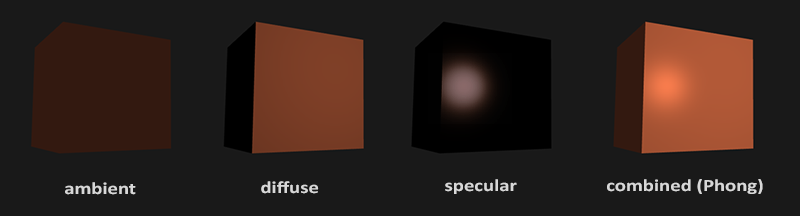
\includegraphics[height = 10 cm, width = 10 cm, keepaspectratio = true]{basic_lighting_phong}
		\caption{Komponente svjetla prikazane na objektu\cite{16}}
		\label{fig:33}
	\end{center}
\end{figure}

\section{Sjenčanje kuglica}
U ovom, posljednjem poglavlju dodati ćemo Shadere koji će osvijetliti kuglice i kuglice koje će biti prozirne i reflektirati svjetlo. U detaljnu analizu samih Shadera nećemo ulaziti. Kodovi koji su napisani su dobro komentirani pa samo objašnjenje Shadera bi bilo suvišno. Shaderi su napisani po uzoru na literaturu\cite{15}. \newpage
\begin{lstlisting}[style = myC++ , label = {code:21}, caption = {Konačni Shader točaka}]
#version 330 core
// Input vertex data, different for all executions of this shader.
layout(location = 0) in vec3 vertexPosition_modelspace;
layout(location = 2) in vec3 vertexNormal_modelspace;
// Output data ; will be interpolated for each fragment.
out vec3 Position_worldspace;
out vec3 Normal_cameraspace;
out vec3 EyeDirection_cameraspace;
out vec3 LightDirection_cameraspace;
// Values that stay constant for the whole mesh.
uniform mat4 VP;
uniform mat4 V;
uniform mat4 M;
uniform vec3 LightPosition_worldspace;
void main(){
  // Output position of the vertex, in clip space : MVP * position
  gl_Position =  VP * M * vec4(vertexPosition_modelspace,1);

  // Position of the vertex, in worldspace : M * position
  Position_worldspace = (M * vec4(vertexPosition_modelspace,1)).xyz;

  // Vector that goes from the vertex to the camera, in camera space.
  // In camera space, the camera is at the origin (0,0,0).
  vec3 vertexPosition_cameraspace = ( V * M * vec4(vertexPosition_modelspace,1)).xyz;
  EyeDirection_cameraspace = vec3(0,0,0) - vertexPosition_cameraspace;

  // Vector that goes from the vertex to the light, in camera space. M is ommited because it's identity.
  vec3 LightPosition_cameraspace = ( V * vec4(LightPosition_worldspace,1)).xyz;
  LightDirection_cameraspace = LightPosition_cameraspace + EyeDirection_cameraspace;

  // Normal of the the vertex, in camera space
  Normal_cameraspace = ( V * M * vec4(vertexNormal_modelspace,0)).xyz; // Only correct if ModelMatrix does not scale the model ! Use its inverse transpose if not.
  }
}
\end{lstlisting}

\begin{lstlisting}[style = myC++ , label = {code:22}, caption = {Konačni Shader fragmenata}]
#version 330 core

// Interpolated values from the vertex shaders
in vec3 Position_worldspace;
in vec3 Normal_cameraspace;
in vec3 EyeDirection_cameraspace;
in vec3 LightDirection_cameraspace;

// Ouput data
out vec4 color;

// Values that stay constant for the whole mesh.
uniform sampler2D myTextureSampler;
uniform mat4 MV;
uniform vec3 LightPosition_worldspace;

void main(){

  // Light emission properties
  // You probably want to put them as uniforms
  vec3 LightColor = vec3(0.8,0.4,0.6);
  float LightPower = 300.0f;

  // Material properties
  vec3 MaterialDiffuseColor = vec3(0.5,0.4,1);
  vec3 MaterialAmbientColor = vec3(0.2,0.7,0.6) * MaterialDiffuseColor;
  vec3 MaterialSpecularColor = vec3(0.4,0.3,0.7);

  // Distance to the light
  float distance = length( LightPosition_worldspace - Position_worldspace );

  // Normal of the computed fragment, in camera space
  vec3 n = normalize( Normal_cameraspace );
  // Direction of the light (from the fragment to the light)
  vec3 l = normalize( LightDirection_cameraspace );
  // Cosine of the angle between the normal and the light direction, 
  // clamped above 0
  //  - light is at the vertical of the triangle -> 1
  //  - light is perpendicular to the triangle -> 0
  //  - light is behind the triangle -> 0
  float cosTheta = clamp( dot( n,l ), 0,1 );

  // Eye vector (towards the camera)
  vec3 E = normalize(EyeDirection_cameraspace);
  // Direction in which the triangle reflects the light
  vec3 R = reflect(-l,n);
  // Cosine of the angle between the Eye vector and the Reflect vector,
  // clamped to 0
  //  - Looking into the reflection -> 1
  //  - Looking elsewhere -> < 1
  float cosAlpha = clamp( dot( E,R ), 0,1 );

  color.rgb = 
  // Ambient : simulates indirect lighting
  MaterialAmbientColor +
  // Diffuse : "color" of the object
  MaterialDiffuseColor * LightColor * LightPower * cosTheta / (distance*distance) +
  // Specular : reflective highlight, like a mirror
  MaterialSpecularColor * LightColor * LightPower * pow(cosAlpha,5) / (distance*distance);
  //Transparency
  color.a = 0.2;
}
\end{lstlisting}\newpage
Nakon dodavanja ovih Shadera kuglica izgleda ovako:
\begin{figure}[!http]
	\begin{center}
		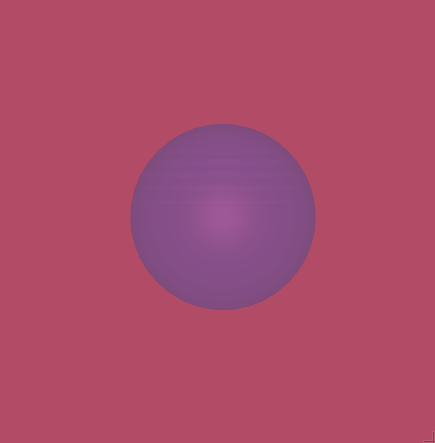
\includegraphics[height = 8 cm, width = 8 cm, keepaspectratio = true]{transparent_sphere}
		\caption{Konačni izgled kuglice sa dodanom prozirnošću}
		\label{fig:34}
	\end{center}
\end{figure}

\section{Zaključno o sjenčanju}
Sama svrha ovoga rada nije bilo dodavanje Shadera. Ovo je dodatni dio koji će samo definirati izgled kuglica i nema nikakve ovisnosti o samom algoritmu za detekciju sudara. Primijetimo da kuglica\ref{fig:34} nije savršena, ali za naše potrebe je bila dovoljna. Sama implementacija OpenGL-a 3.3 oduzela je dosta vremena, no na kraju dobili smo rad koji ima nekakav izgled, a ne samo bijele kuglice na crnoj podlozi. Shaderi su moćan alat kojime se može ubrzati i broj sličica po sekundi ako su dobro definirani\cite{15}. U našem slučaju samo crtanje nam nije ubrzalo algoritam pa je još uvijek crtanje sa velikim brojem kuglica bilo problematično zbog složenosti algoritma za detekciju sudara.